%% LaTeX2e class for student theses
%% thesis.tex
%% 
%% Karlsruhe Institute of Technology
%% Institute for Program Structures and Data Organization
%% Chair for Software Design and Quality (SDQ)
%%
%% Dr.-Ing. Erik Burger
%% burger@kit.edu
%%
%% See https://sdqweb.ipd.kit.edu/wiki/Dokumentvorlagen
%%
%% {$HeadURL: https://svnserver.informatik.kit.edu/i43/svn/lehre/Abschlussarbeiten-Vorlage/thesis.tex $}
%% {$LastChangedDate: 2018-08-02 14:19:06 +0200 (Do, 02 Aug 2018) $}
%% {$LastChangedRevision: 5705 $}
%% {$LastChangedBy: burger $}

%% Available page modes: oneside, twoside
%% Available modes: draft, final (see README)
\documentclass[twoside, english, draft]{sdqthesis}

%% ---------------------------------
%% | Information about the thesis  |
%% ---------------------------------

%% Name of the author
\author{Hannes F. Kuchelmeister}

%% Title (and possibly subtitle) of the thesis
\title{Decision Support for Group-Based Configuration using Recommender Systems}

%% Type of the thesis 
\thesistype{Bachelor's Thesis}

%% Change the institute here, ``IPD'' is default
% \myinstitute{Institute for \dots}

%% You can put a logo in the ``logos'' directory and include it here
%% instead of the SDQ logo
% \grouplogo{myfile}

%% Alternatively, you can disable the group logo
\nogrouplogo

%% The reviewers are the professors that grade your thesis
\reviewerone{Prof. Dr. Ralf H. Reussner}
\reviewertwo{Prof. Dr. Christof Weinhardt}

%% The advisors are PhDs or Postdocs
\advisorone{Dr. rer. nat. Robert Heinrich}
%% The second advisor can be omitted
\advisortwo{M.A. Jonas Fegert}

%% Please enter the start end end time of your thesis
\usepackage{texdate}
\initdate{2019}{12}{16}

\editingtime{
    \printfdate{british}
}{
    \advancebymonths{4}
    \advancebydays{34} % corona automatic extension
    \printfdate{british}
}

\settitle

%% --------------------------------
%% | Settings for word separation |
%% --------------------------------

%% Describe separation hints here.
%% For more details, see 
%% http://en.wikibooks.org/wiki/LaTeX/Text_Formatting#Hyphenation
\hyphenation{
% me-ta-mo-del
}

%% --------------------------------
%% | Ref Hypothesis                 |
%% --------------------------------
\newcommand{\hypothesisautorefname}{Hypothesis}

%% --------------------
%% |  Float Barriers  |
%% --------------------
\usepackage{placeins}

%% --------------------
%% |  Table Packages  |
%% --------------------
\usepackage{tabularx}
\usepackage{multirow}

%% --------------------
%% |  Maths Packages  |
%% --------------------
\usepackage{amsmath}
\usepackage{amssymb}

%% --------------------
%% | Plotting Packages |
%% --------------------
\usepackage{pgfplots}

%% ---------------------
%% | Generating Frames |
%% ---------------------
\usepackage[framemethod=TikZ]{mdframed}
\mdtheorem[
    linecolor=gray!60,
    linewidth=1pt,
    frametitlebackgroundcolor=gray!20,
    frametitlefont=\sffamily\bfseries\color{black},
]{hypothesis}{Hypothesis}[section]

%% --------------------------------
%% | PDF Comments                 |
%% --------------------------------
\usepackage[colorinlistoftodos, obeyDraft]{todonotes}


%% --------------------------------
%% | Gantt Charts                 |
%% --------------------------------
\usepackage{pgfgantt}

%% --------------------------------
%% | Quotation                 |
%% --------------------------------

\usepackage{csquotes}
\MakeOuterQuote{"}

%% --------------------------------
%% | Bibliography                 |
%% --------------------------------

%% Use biber instead of BibTeX, see README
\usepackage[citestyle=numeric,style=numeric,sorting=none,backend=biber]{biblatex}
\addbibresource{thesis.bib}

%% --------------------------------
%% | File Inputs                 |
%% --------------------------------
\usepackage{texosquery}

%% ====================================
%% ====================================
%% ||                                ||
%% || Beginning of the main document ||
%% ||                                ||
%% ====================================
%% ====================================
\begin{document}

%% Set PDF metadata
\setpdf

%% Set the title
\maketitle

%% The Preamble begins here
\frontmatter

%% LaTeX2e class for student theses: Declaration of independent work
%% sections/declaration.tex
%% 
%% Karlsruhe Institute of Technology
%% Institute for Program Structures and Data Organization
%% Chair for Software Design and Quality (SDQ)
%%
%% Dr.-Ing. Erik Burger
%% burger@kit.edu
%%
%% Version 1.3.3, 2018-04-17

\thispagestyle{empty}
\null\vfill
\noindent\hbox to \textwidth{\hrulefill} 
\iflanguage{english}{I declare that I have developed and written the enclosed
thesis completely by myself, and have not used sources or means without
declaration in the text.}%
{Ich versichere wahrheitsgemäß, die Arbeit
selbstständig angefertigt, alle benutzten Hilfsmittel vollständig und genau
angegeben und alles kenntlich gemacht zu haben, was aus Arbeiten anderer
unverändert oder mit Änderungen entnommen wurde.}
 
 
%% ---------------------------------------------
%% | Replace PLACE and DATE with actual values |
%% ---------------------------------------------
\todo[inline]{Replace PLACE and DATE with actual values}
\textbf{PLACE, DATE}
\vspace{1.5cm}
 
\dotfill\hspace*{8.0cm}\\
\hspace*{2cm}(\theauthor) 
\cleardoublepage


\setcounter{page}{1}
\pagenumbering{roman}

%% ----------------
%% |   Abstract   |
%% ----------------
 
%% For theses written in English, an abstract both in English
%% and German is mandatory.
%%
%% For theses written in German, a German abstract is sufficient.
%%
%% The text is included from the following files:
%% - sections/abstract

\includeabstract

%% ------------------------
%% |   Table of Contents  |
%% ------------------------
\tableofcontents

\listoffigures
\listoftables

%% -----------------
%% |   Main part   |
%% -----------------

\mainmatter

\chapter{Introduction}
\label{ch:Introduction}

\section{Problem}
\label{sec:Introduction:Problem}

A group of people with different personal preferences wants to find a solution to a problem with high variability. Making decisions in the group comes with problems as a lack of communication leads to worse decision outcomes \cite{atasItemRecommendationUsing2017}. Group dynamics and biases can lead to suboptimal decisions \cite{kerrBiasJudgmentComparing1996}. Generally group decisions are complex and often the process that yields the decision result is unstructured, thereby not providing any reproducibility of the success. Groups have different power structures and usually individuals have different interests. Moreover finding solutions is a rather complex task and group decisions can suffer intransparency.

Examples of group recommendation decisions are:
\begin{itemize}
    \item A companies truck fleet (e.g. driver, purchasing-manager, marketing manager)
    \item A companies customer management software system (e.g. salesperson, human resource manager, accounting manager)
    \item A public project to get a new area at a zoo (e.g. visitor, director, animal keeper)
    \item Managing a forest (e.g. owner, environmental protection agency, consumer representative)
    \item An existing company building and how it should be furnished (e.g. landlord, employee representative, CEO)
\end{itemize}

These examples are different from an ordinary group decision in the sense that the components the solution is build from are standardised but a solution is highly individual because of high variability. The solution space therefore is rather large.

\section{Idea}
\label{sec:Introduction:Idea}

To support groups in their decision making product configuration can be used. It allows to accurately map constraints and dependencies in complex problems and to map the solution space. Using a group recommender a group is supported in their configuration decisions. The goal is to show that these approaches can help a group with the configuration task presented by the usage of a configurator and to better process individual preferences than a human can.


There does not exists much research on recommendation for group configuration, however it is comprised of two different areas of research, recommenders for groups and recommenders for configuration.
The existing literature on recommenders for groups is extensive with many different approaches and domains \cite{delicResearchMethodsGroup2016, chenInterfaceInteractionDesign2011, atasItemRecommendationUsing2017, jamesonRecommendationGroups2007, chenEmpatheticonsDesigningEmotion2014, liuCGSPAComprehensiveGroup2019}. \citeauthor{felfernigGroupRecommenderSystems2018} give an overview about basic approaches \cite{felfernigGroupRecommenderSystems2018}.
In the area of product configuration research about recommender systems is undertaken as well \cite{pereiraFeatureBasedPersonalizedRecommender2016, scholzConfigurationbasedRecommenderSystem2017, scholzEffectsDecisionSpace2017}.
Group configuration is a more specialized sub field of configuration therefore less attention has been directed towards it and because of that there has not been much research on recommenders that are for group recommendation in a configuration setting.

\section{Benefits}
\label{sec:Introduction:Benefits}

The benefits of this approach are, that the need for a group to communicate directly is reduced. Each user gives their own preferences and the group will get a recommendation based on that. This allows to reduce problems arising in groups decisions like lack of communication and bias in groups. Additionally this shows the viability of combining group recommendations and configuration approaches.

\section{Action}
\label{sec:Introduction:Action}

As resulting action in this thesis a prototype will be designed, implemented and evaluated that achieves the following objectives.
\begin{itemize}
    \item A system should give recommendation for the group using a scoring function that takes into account preferences of group members and the current state of the situation.
    \item Recommendations should allow different scoring functions.
    \item Recommendations should always be valid options.
    \item The system should consider all preferences of individuals in a group and find a solution that most people of the group are happy with.
\end{itemize}
The results are communicated through this thesis. Thereby adhering to the research method of design science research \cite{peffersDesignScienceResearch2007}.
\chapter{Foundations}
\label{ch:Foundations}

Since this thesis focuses on recommender systems to support group decisions in the context of group based configuration it is important to define what we mean by these terms. This chapter describes foundations that sow what a recommender system is, approaches that can be taken and how it is possible to build with these approaches a group recommender. Additionally configuration and group configuration are defined. In group decisions biases can have an effect of the groups decision making ability and some of these are presented here to consider their effect on group decisions. 

\section{Recommender System}
\label{sec:Foundations:RecommenderSystem}

A recommender system is a system that gives individualized recommendations to users to guide them through a large space of objects \cite[~ p. 331]{burkeHybridRecommenderSystems2002}.

There are several approaches to recommender systems presented in \cite{felfernigGroupRecommenderSystems2018}, these are: collaborative filtering, content-based filtering, critiquing-based filtering, constraint-based, hybrid recommendation.

\begin{table}
    \centering    
    \begin{tabular}{ l | c | c | c | c | c }
        & The Matrix & Titanic & Die Hard & Forest Gump & Wall-E \\ \hline
         John  & 5 & 1 &   & 2 & 2 \\
         Lucy  & 1 & 5 & 2 & 5 & 5 \\
         Eric  & 2 & ? & 3 & 5 & 4 \\
         Diane & 4 & 3 & 5 & 3 &   \\
    \end{tabular}
    \caption{An example showing users ratings for movies by \citeauthor{ningComprehensiveSurveyNeighborhoodBased2015} \cite{ningComprehensiveSurveyNeighborhoodBased2015}.}
    
    \label{tab:Foundations:RecommenderSystem:MoviePreferences}
\end{table}

\subsection{Collaborative Filtering}
In collaborative filtering a users rating for unknown items is predicted by finding similar users who have rated it. Their rating is used as prediction
\cite[~ pp. 7, 8]{felfernigDecisionTasksBasic2018}.

Collaborative Filtering can not only be done using users, it can also be item-based. Hereby the similarity between items is used for a recommendation and not similar users \cite{ricciRecommenderSystemsHandbook2015}. In the context of configuration the similarity to other historic configurations can be used which makes it an item based approach. 

Table \ref{tab:Foundations:RecommenderSystem:MoviePreferences} shows an example rating matrix. A simple user-based way to calculate rating would be now to use a k-nearest neighbour (kNN) algorithm and then take the average of those ratings. Using this method with $k := 2$ and euclidean distance our closest neighbours are \textit{Lucy} and \textit{Diane} therefore giving us a predicted rating of $4$.  If we use item based illustration instead, we will try to find similar items based on the users rating. An example of similar items here would be \textit{Forest Gump} and \textit{Wall-E} as John and Lucy each have given them the sane rating and Eric's rating is off by one. Using again kNN with $k := 2$ we find that \textit{Forest Gump} and \textit{Wall-E} are the most similar to \textit{Titanic} thereby having a predicted rating of $4.5$.
However this simple similarity and prediction function does not take into account different distances. For example Lucy's ratings are more similar compared to Eric's than Diane's but Diane's and Lucy's rating is valued the same amount.

\subsection{Content-Based Filtering}
Items and users are assigned to categories. Based on consumption and rating of items a user will have implicit ratings for categories. Predictions are now made based on a categories of the new item \cite[~ pp. 10, 11]{felfernigDecisionTasksBasic2018}.

Using our example from Table \ref{tab:Foundations:RecommenderSystem:MoviePreferences} and using an additional category matrix (see Table \ref{tab:Foundations:RecommenderSystem:ContentBasedFilteringCategories}) we can derive a rating matrix per category (using the average rating of the user of each movie contained in this category). The result can be seen in Table \ref{tab:Foundations:RecommenderSystem:ContentBasedFilteringProfiles}. To predict Eric's rating of Titanic we now can use the categories of \textit{Titanic} and average out Eric's implicit rating per category. Titanic is only in the category romance and as Eric's rating of \textit{Forest Gump} is $5$ the prediction is a rating of $5$. Categories don't have to be the genre, they could be any kind of data about a movie.

\begin{table}
    \centering    
    \begin{tabular}{ l | c | c | c | c | c }
        & The Matrix & Titanic & Die Hard & Forest Gump & Wall-E \\ \hline
         Action  & x &  & x  &  &  \\
         Sci-Fi  & x &  &  &  &  \\
         Thriller  &  & & x &  &  \\
         Romance & & x & & x & \\
         Family & & & & x & x \\
    \end{tabular}
    \caption{Showing example categories for movies in Table \ref{tab:Foundations:RecommenderSystem:MoviePreferences}.}
    
    \label{tab:Foundations:RecommenderSystem:ContentBasedFilteringCategories}
\end{table}

\begin{table}
    \centering    
    \begin{tabular}{ l | c | c | c | c | c }
        & Action & Sci-Fi & Thriller & Romance & Family \\ \hline
        John  & 5 & 5 & & 1.5 & 2 \\
        Lucy  & 1.5 & 1 & 2 & 5 & 5 \\
        Eric  & 2.5 & 2 & 3 & 5 & 4.5 \\
        Diane & 4.5 & 4 & 5 & 3 & 3  \\
    \end{tabular}
    \caption{User profiles generated from categories and rating from Tables \ref{tab:Foundations:RecommenderSystem:MoviePreferences} and \ref{tab:Foundations:RecommenderSystem:ContentBasedFilteringCategories}.}
    
    \label{tab:Foundations:RecommenderSystem:ContentBasedFilteringProfiles}
\end{table}

\subsection{Critiquing-Based Recommendation}
Items are recommended and a user can then critique on attributes of the recommendation. Based on that a similar item which does not have those critiques can be recommended. User preferences are implicitly collected this way \cite{knijnenburgEachHisOwn2011}.

With a critique based approach Eric sees a suggestion of watching \textit{The Island} and its attributes. He then can say that he finds this movie has too much action. The critique based recommender will now present a movie that has similar attributes as \textit{The Island} but with less action. For example \textit{Titanic} could be the next suggestion.

\subsection{Constraint-Based Recommendation}
Hereby filter rules are defined which filter out items that don't fulfil specified rules. A user models their requirements with these rules and thereby gets a list of recommended items. This approach requires deep knowledge about a product because it needs a detailed description of features  \cite[~ p. 12]{felfernigDecisionTasksBasic2018}.

Our movie example (see Table \ref{tab:Foundations:RecommenderSystem:MoviePreferences}) needs have additional information for example about plot structure, pacing, length and other attributes of the movie. Now the user could give as filter, that the movie should be no longer than 120 minutes, be categorized as action or thriller and have a fast pacing. The system will only recommend movies that fit into these categories.

\subsection{Hybrid Recommendation}
A hybrid recommender combines different recommendation approaches to use the strengths of each individual one and to reduce effects of weaknesses \cite{burkeHybridRecommenderSystems2002}.

\section{Group Recommender System}

A group recommender system is a recommender system aimed at making recommendations for a group instead of a single user. To make recommendations group members preferences have to be aggregated. This can be done by either aggregating single user recommendations or by merging preferences of each user into a group preference model. Based on this model recommendation strategies as described in \ref{sec:Foundations:RecommenderSystem} can be used to generate recommendations \cite{jamesonRecommendationGroups2007}.

\section{Product Configuration}
\label{sec:Foundations:ProductConfiguration}

Product configuration is a process consisting of a series of decision tasks whereby a product is constructed of components which interact with each other. During a configuration process no new components are created. Their interplay and specification is defined beforehand \cite[~ pp. 42, 43]{sabinProductConfigurationFrameworksa1998}.

Formally a configuration problem can be specified as a \emph{constraint satisfaction problem (CSP)} \cite{tsangFoundationsConstraintSatisfaction1993} as 
\[
    CSP(V,D,C)
\]
where \( V = \{v_1,\dots, v_n\} \) is a set of variables, \( D = dom : V \mapsto X \) is a relation of variables and their corresponding domain definitions \( X \), and \( C = C_{PREF} \cup C_{KB} \) is a set of constraints with customer preferences \( C_{PREF} \) and configuration knowledge base \( C_{KB} \) \cite{felferningGroupBasedConfiguration2016, felfernigOpenConfiguration2014}.


\section{Group-Based Product Configuration}
\label{sec:Foundations:GroupBasedProductConfiguration}

If instead of a single person configuring a product we would like to have a group of people which can be useful in multi-stakeholder decisions, it needs mechanisms for describing the preferences of multiple people. Therefore we extend the definition of product configuration from (\ref{sec:Foundations:ProductConfiguration}) to 
\[ 
    C_{PREF} = \bigcup 
PREF_i \]
with preferences of user \( i \) as \( PREF_i \) \cite{ felferningGroupBasedConfiguration2016}.

\section{Group-Based Configuration-Solution}
\label{sec:Foundations:GroupBasedConfigurationSolution}

\ref{sec:Foundations:ProductConfiguration} and \ref{sec:Foundations:GroupBasedProductConfiguration} expand to a solution of a group-based configuration with the addition of variable assignments
\[
    C_{CONF} = \bigcup_{v_i \in V} \{ v_i = x_i \}, \ x_i \in dom(v_i)
\]
and where \( C_{CONF} \cup C_{PREF} \cup C_{KB} \) is consistent \cite{ felferningGroupBasedConfiguration2016}.

\section{Group Bias}
\label{sec:Foundations:GroupBias}

Groups have biases same as individuals. Some of these stem from individual biases that are transferred to a group and others only occur in group settings. This section covers some of those effects. These effects are described by \citeauthor{felfernigBiasesGroupDecisions2018} \cite{felfernigBiasesGroupDecisions2018}.

\subsection{GroupThink}

The bias called GroupThink occurs, when group members prefer to avoid conflicts instead of being mainly interested in getting the best decision outcome. Alternative options are in these circumstances not analysed close enough \cite{janis1982groupthink}.
An avoidance strategy for this effect is for leaders to delay stating there opinion until all alternatives have been viewed in detail \citeauthor{felfernigBiasesGroupDecisions2018}. Recommender systems can aid group decision quality through encouraged information exchange as discussed by \citeauthor{atasItemRecommendationUsing2017} in \cite{atasItemRecommendationUsing2017}.


\subsection{Anchoring}

The first information provided is relied upon to heavily. In a group setting this can be triggered by the group member to first express their opinion. Often this is triggered if group members see preferences of others too early, therefore recommender systems should not show the rating of other users \cite{cosley2003seeing}.

\subsection{Serial Position Effects}

The serial positioning effects is the effect that users have a higher retention rate of items in a list that are presented first or last and these items are more closely examined \cite{felfernigPersuasiveRecommendationSerial2007,murphyPrimacyRecencyEffects2006}. Additionally to remembering and examining items at the start and the end of a list also the order of items can change the option the user chooses in the end \cite{felfernigBiasesGroupDecisions2018}.



\chapter{Related Work}
\label{ch:RelatedWork}

\chapter{Concept}
\label{ch:Concept}

In this chapter definitions from \autoref{ch:Foundations} are extended, requirements formulated and assumptions made. Later, user interaction with the recommender system is described and the case study presented. Moreover, the process of generating recommendations is formulated and described. Last, the concept is illustrated using an example.

\section{Foundations Extension}
\label{sec:Concept:Requirements}

The definitions described in \autoref{ch:Foundations} need to be extended for this thesis. This section adds definitions that are required.

\subsection{Configuration State}

A \emph{configuration} $S$ will be defined as a tuple of variables (\autoref{eq:Foundations:ProductConfiguration:Variables}) and their corresponding domain value with
\begin{equation} \label{eq:Foundations:ProductConfiguration:ConfigurationState}
    S = \{ (v_i,\ d) \ |\ v_i \in V \ \land \ d \in \mathfrak{D}(i),\ i=1,\dotsc,m \}.
\end{equation}
Essentially it is a set of variables and assigned values.

\subsection{Finished Configuration}
To define what a \emph{finished configuration} is, it is necessary to first define what it means for a configuration to be valid. Therefore $is\_valid$ is defined as
\begin{equation} \label{eq:Foundations:ProductConfiguration:IsValid}
    is\_valid : S \to \{true, false\}; x \mapsto 
    \begin{cases}
        true, & S \in solution\_space \\
        false, & \text{otherwise}
    \end{cases},
\end{equation}
with $solution\_space$ being the solution space of the corresponding constraint satisfaction problem. A \emph{finished configuration} $S_F$ is a configuration that contains all variables and is a valid configuration:
\begin{equation} \label{eq:Foundations:ProductConfiguration:FinishedConfiguration}
    S_F \subset S,\ where \ \forall v_i \in V (\exists (v_i, d) \in S_F : d \in \mathfrak{D}(i)) \land is\_valid(S_F).
\end{equation}
In practice, a finished configuration of a product is something that is ready to be produced. For example if a car is being configured, this means that the car can be produced in the specified way given by the finished configuration.


\subsection{Group-Based Product Configuration}
\label{sec:Foundations:GroupBasedProductConfiguration}

Instead of a single person configuring a product, a group of people configures one product which can be useful in multi-stakeholder decisions. This setting needs mechanisms for describing the preferences of multiple people. Therefore, a set of users $U$ will be introduced with
\begin{equation}\label{eq:Foundations:ProductConfiguration:Users}
    U = \{1, \dotsc, n\},
\end{equation}
and a user's \emph{utility function} that maps a domain value to a utility value and is only known to the user
\begin{equation}
    \begin{split}
        u_i(d_j), \qquad \text{where}\ & u_i(d_j) \in [0,1] \\
        & d_j \in  \mathfrak{D}(j),\\
        & 1 <= j <= m, \\
        & 1 <= i <= n.
    \end{split}
\end{equation}

\subsection{Group Recommender}

For a group recommender system additional definitions are required. The attitude of users is represented by their preferences $P$ which are directly related to how the user benefits from a domain value being present in the configuration. Let 
\begin{gather} \label{tab:Foundations:GroupRecommenderSystem:Preferences}
    P = \{ P_1, \dotsc, P_n\},\ \text{where} \\
    P_i = \{(d,\ u_i(d)) \ | \ \forall d \in \mathfrak{D}(i),\ i=1,\dotsc,m \} \notag
\end{gather}


\section{Requirements}
\label{sec:Concept:Requirements}

This section lists requirements that are considered and implemented in this thesis by the group-based configurator, including the recommendation system.

\begin{itemize}
    \item Mandatory:
        \begin{itemize}
            \item The recommender should support a continuous value range for preferences
            \item The recommendation engine can be used without proprietary software.
            \item Give recommendations to a group, based on their preferences and the current configuration state.
            \item The system supports multiple group configurators at the same time.
            \item The system should take the current configuration state into account.

            \item Recommendations should always be valid solutions.
            \item The system has to respond in a timely manner.
        \end{itemize}
    \item Optional:
        \begin{itemize}
            \item Provide a simple user interface.
            \item The system should be able to work with other configuration systems.
            \item Recommendations should allow different scoring functions.
        \end{itemize}
\end{itemize}


\section{Assumptions}
\label{sec:Concept:Assumptions}

Due to the fact that a thesis has limited resources, some assumptions have to be made. The assumptions made are listed in this section.

\begin{itemize}
    \item Only one product/solution is supposed to be configured at the same time by one group.
    \item Features only support single value attributes.
    \item Users join the system and start configuring only after all group members have joined.
    \item Speed and optimization of the system does not have high priority.
    \item The user interface is for demo purposes.
\end{itemize}
In order to reduce complexity, the assumptions are made that only single value attributes are supported and one product is configured at a time by a group. Therefore, less implementation work is needed. However, results are not dependent on these implementations. Most features use only single value attributes. It is also possible to model a feature that supports multiple attributes. As an example the feature \emph{audio system} has the following options: \emph{Bluetooth} or \emph{CD}. To allow multiple attributes to be selected the characteristics \emph{Bluetooth and CD} can be added.
The assumption that users join the system and only start configuring once all members of the group joined is made to reduce the amount of work needed for creating a lobby and waiting system which is not relevant for showing the functionality of the recommender. Speed and optimization of the system having no high priority as the speed has no influence on the results of this thesis. Therefore, as long as the system is fast enough, no further optimisation of speed is needed.
The evaluation is done solely with the recommender system and its APIs. Thus, the user interface is not directly relevant for the evaluation but it is relevant for communication of results.

\section{User Interaction with the System}
\label{sec:Concept:UserSystemInteraction}

The system has one main way to be used as defined in \autoref{tab:Concept:MainUseCase}. This process is also visualized in \autoref{fig:Concept:ConfigurationProcess}. All users start the configuration process together.
They select the current state at the beginning of the process. Then repeatedly users enter their preferences until each user's preference have been entered into a system. Based on the entered preferences the system generates a recommendation that is a compromise of all users preferences.

\begin{figure}
    \centering
    \includegraphics[width=1\textwidth]{./figures/40_concept/bpmn_configuration_process_with_continious_recommendation.pdf}
    \caption{A BPMN diagram of the configuration process.}
    \label{fig:Concept:ConfigurationProcess}
\end{figure}

\begin{table}
    \begin{center}
        \begin{tabularx}{\columnwidth}{l|X}
            \multicolumn{2}{c}{Main System Usage} \\
            \hline
            Preconditions   & 
                \begin{itemize}
                    \item The configurator is opened with the same session on each of the group member's machines
                    \item The configuration is in an unfinished state (this state is a consensus state)
                \end{itemize} \\
            \hline
            Postcondition   & 
                \begin{itemize}
                    \item All users have entered their preferences for each attribute explicitly.
                    \item The system gives a recommendation based on all preferences and the unfinished configuration state
                \end{itemize} \\
            \hline
            Basic Flow      & 
                \begin{enumerate}
                    \item A user indicates a preference for an attribute
                    \item The system generates a recommendation (based on preferences and configuration status)
                    \item If not all users have given their preferences go to step 1.
                \end{enumerate} \\
            \hline
        \end{tabularx}
        \caption{A description of the main way users will interact with the system}
        \label{tab:Concept:MainUseCase}
    \end{center}
\end{table}

\section{Case Study}
\label{sec:Concept:CaseStudy}

The case study used in this thesis is a simplified version from forestry \todo[]{hier evtl ergänzen: wo kommt der Use Case her / aus welchem Forschungsprojekt / warum ist er interessant?}.
The used characteristics and attributes are shown in \autoref{fig:Concept:ForestExample}. Additionally, as examples preferences, a configuration state and a finished configuration are given.

\begin{figure}
    \begin{mdframed}[frametitle={Example for Forest Use Case}, linecolor=black, frametitlerulecolor=black, frametitlebackgroundcolor=gray!5]
        In this example there is a small group of users. The use case is a piece of forest and variables are for example harvesting activity, which trees to grow and accessibility for people.
        \begin{align}
            \begin{split}
                V = \{ & \textit{indigenous}, \textit{resilient}, \textit{usable}, \textit{effort}, \textit{quantity}, \textit{price}, \textit{accessibility} \},
            \end{split} \notag \\
            \mathfrak{D}(\textit{indigenous}) =  \{ & \text{low}, \text{moderate}, \text{high}\}, \notag \\
            \mathfrak{D}(\textit{resilient}) = \{ & \text{low}, \text{moderate}, \text{high}\}, \notag \\
            \mathfrak{D}(\textit{usable}) = \{ & \text{low}, \text{moderate}, \text{high}\}, \notag \\
            \mathfrak{D}(\textit{effort}) = \{ & \text{manual}, \text{harvester}, \text{autonomous}\}, \notag \\
            \mathfrak{D}(\textit{quantity}) = \{ & \text{low}, \text{moderate}, \text{high}\}, \notag \\
            \mathfrak{D}(\textit{price}) = \{ & \text{low}, \text{moderate}, \text{high}\}, \notag\\
            \mathfrak{D}(\textit{accessibility}) = \{ & \text{low}, \text{moderate}, \text{high}\},\notag \\
            U = \{ & 1,2\} \notag\\
            P = \{ & P_1, P_2\} \notag\\
            \begin{split}
                P_1 = \{ & (\text{manual}, 0.8), (\text{harvester}, 0.3) \} \\ 
                & \cup \{ (d,0.5)\ |\ d \in \mathfrak{D}(i),\ i \in V,\ i \notin \{ \text{manual}, \text{harvester}\} \ \} \ 
            \end{split} \notag \\
            P_2 = \{ & (d,0.5)\ |\ d \in \mathfrak{D}(i),\ i \in V \} \notag \\
            S  =  \{ & (\textit{indigenous}, \text{low}), (\textit{quantity}, \text{moderate}) \} \notag \\
            \begin{split}
            S_F  =  \{ & (\textit{indigenous}, \text{low}), (\textit{resilient}, \text{low}), (\textit{usable},\text{low}), (\textit{effort}, \text{manual}), \\
            & (\textit{quantity}, \text{low}), (\textit{price},\text{high}),(\textit{accessibility}, \text{low}) \} 
            \end{split} \notag
        \end{align}
    \end{mdframed}
    \caption{An example of a forest use case that includes two people.}
    \label{fig:Concept:ForestExample}
\end{figure}


\section{Recommendation Generation}
\label{sec:Concept:SolutionGeneration}

This section describes how recommendations are generated. The recommender system has a database that stores possible finished configurations and the goal is to rank these recommendations according to a scoring function and to recommend the best possible configuration. The scoring function is referred to as the \emph{group configuration scoring function}. It uses the current configuration state, the preferences of the group and a finished configuration to calculate a score. This score resembles how good this configuration resembles the interest of the group. The exact procedure looks as follows:

\begin{enumerate}
    \item Assign a score to each stored configuration according to $$score_{group}(\overline{configurationState},\ \overline{preferences}, \ configurationInStore)$$
    \item Chose the configuration with the highest score as recommendation.
\end{enumerate}

It is optionally possible to have multiple runs with different scoring functions. This, for example, allows the removal of configurations that cause a lot of misery.



\subsection{Scoring Function}

\label{subsec:Concept:SolutionGeneration:ScoringFunction}

The \emph{group configuration scoring function} includes preferences and current configuration state. This function gives a score for a finished configuration (while using the current configuration state and all user preferences):
\begin{equation}
    score_{group}: S \times P \times S_F \to \mathbb{R}
\end{equation}

An example group configuration scoring function is $score_{group}$ with
\begin{equation}
    score_{group}(\overline{s},\ \overline{p},\ s) = score(\overline{p},\ s) \cdot penalty(\overline{s},\ s)
\end{equation} 

This thesis will use multiple scoring functions. Among those are ones for least misery, average and multiplicative which all are implemented by $score$ (see \autoref{subsec:Concept:ReccomendationGeneration:PreferenceScoring} and \autoref{subsec:Concept:ReccomendationGeneration:Penalty}). Average and multiplicative yield good results among the studies presented by \citeauthor{Masthoff2015} \cite{Masthoff2015}. Strategies can also be combined, one example here is average without misery. The scoring functions used for this thesis all combine $penalty$ and $score$ by multiplication. However it is possible to use other combination strategies and it is possible to combine multiple scoring functions into one group scoring function. This thesis will use simpler scoring functions that are not combined but improvement here is possible.

\subsection{Preference Scoring}
\label{subsec:Concept:ReccomendationGeneration:PreferenceScoring}

All of the aggregation functions mentioned in \autoref{subsec:Concept:SolutionGeneration:ScoringFunction} have one preference per product. For configuration where a preference for all characterises exists there needs to be a function that combines the preferences of one user into her configuration score. After one score has been calculated per user the mentioned preference aggregation strategies can be used.

A simple scoring function approach is to use the the preference for each characteristic that is part of the configuration and then use the average. This approach is transparent because the preference of a user is directly translated into the score and no weighting is done. It means that a configuration score is simple to understand and to calculate. However, if needed, for example, to give one group member more power, it allows relative weighting. This can be done with preprocessing of preferences. Moreover, an approach like this ensures that through preprocessing feature weights can be added. It is therefore possible that a user gives different importances to features. Also, other means of weighting ratings are possible. For example the ratings of one group member who has more knowledge in an area can be increased by multiplication with a factor or alternatively the preferences for all other users can be decreased.
The formula for this rating function looks as follows:

\begin{equation}
    score(\overline{p},\ s) = aggr( \ \{score_{user}(P_i, s) \ | \ P_i \in \overline{p} \} \ )
\end{equation}
where $aggr$ the aggregation function and $score_{user}(P_i, s)$ the configuration score of user $i$ which is defined as
\begin{equation}
    score_{user}(P_i, s) = average(\{x \ | \ (characteristic, x) \in P_i \land characteristic \in s \}) \notag . 
\end{equation}

The example in \autoref{fig:Concept:ForestExample} contains two users. The first user has preferences for the characteristic \emph{manual} of the feature with $0.8$ and the characteristic \emph{harvester} of the same feature with $0.3$. All other characteristics have a preference of $0.5$. The second user's preferences are $0.5$ for all characteristics. The finished configuration that is supposed to be rated in this example contains the characteristics \emph{low} for each feature except for \emph{effort} and \emph{quantity} which are set to \emph{manual} and \emph{high}. The score fore the finished configuration $S_F$ of user one is $0.54$. This score is the average of all seven features. User one rates all characteristics of all features as $0.5$ except two characteristics for \emph{effort}. Therefore all, feature scores for this user are $0.5$ except the score for \emph{effort} is $0.8$ because of the user's preference of $0.8$ for the characteristic \emph{manual}. The resulting average score per feature of $0.54$ is the user's score for this configuration. User two rates all characteristics with $0.5$ therefore the resulting average is $0.5$.
The group configuration score is dependent on the used aggregation strategy. Multiplication results in a score of $0.54 \cdot 0.5 = 0.27$. The score for average is $\frac{1}{2}(0.54 + 0.5) = 0.52$ and for least misery $\min \{0.54, 0.5\} = 0.5$.

\subsection{Configuration Change Penalty}
\label{subsec:Concept:ReccomendationGeneration:Penalty}

In this thesis a penalty function is proposed which gives the percentage of characteristics that exist in the configuration that is to be rated. This value can be tuned to be more or less strict by potentiating. This is done by selection different values for $\alpha$. Thereby allowing more deviation or less deviation from the current configuration state. The penalty function is defined as
\begin{equation}
    \notag \alpha \in \mathbb{R}, \qquad     unchanged(d,\overline{s}, s) = 
    \begin{cases}
      1, & d \in \overline{s} \land d \in s \\
      0, & \text{otherwise}
    \end{cases}
\end{equation}

\begin{equation}
    penalty_{proportion}(\overline{s},\ s) =  \left(\frac{\sum_{d \in \overline{s}} unchanged(d,\overline{s}, s)}{|\overline{s}|}\right)^\alpha.
\end{equation}
In essence the the function checks the number of unchanged characteristics and divides this by the number of characteristics that are in the current configuration state. The result is the proportion of unchanged characteristics when comparing the current configuration state to the finished configuration.

By including the current configuration state, the scoring function can take into account that some characteristics have already been realized and therefore might be very costly to change. A higher $\alpha$ resembles a higher cost of change and an alpha of zero represents no costs for changes.

\section{Illustration}
\label{sec:Concept:Illustration}

This section gives an example to illustrate how the recommendation works. The example in \autoref{fig:Concept:ForestExample} is used for that but the preferences are extended. \autoref{tab:Concept:UseCaseConfigurations} shows the current configuration state which consists of the characteristic moderate for the feature \textit{indigenous} and  \textit{resilient} respectively. $S_{F1}$ to $S_{F4}$ show the stored configurations for this example. The features that will be focused on are \textit{indigenous}, \textit{resilient} and \textit{effort}. In the presented example $S_{F1}$ performs best. The exact reason for that will be presented here. $S_{F1}$ is compared to $S_{F2}$ to show the effect of divergence from the configuration state.  A comparison between $S_{F1}$  and $S_{F3}$ is done to show the difference between preferences and the effect on the score and last, $S_{F4}$ is done to show the effect of switching to better preferences but diverging from the current state. The configurations all differ to $S_{F1}$ in only one characteristic that is chosen differently. As aggregation strategy the \emph{average} metric is used (see \autoref{sec:Foundations:GroupRecommenderSystem}). The parameter $\alpha$ (see \autoref{subsec:Concept:ReccomendationGeneration:Penalty}) is set to 1. A lower $\alpha$ reduces the penalty given to configurations that deviate from the configuration state $S$ and a higher $\alpha$ increase the reluctance to change.

The difference between  $S_{F1}$ and  $S_{F2}$ is that instead of containing \emph{moderate} for the feature \emph{resilient} $S_{F2}$ contains \emph{high}. The scores for these two characteristics are the same, with a value of $0.55$, as both users have rated them at $0.5$ but since $S_{F2}$ deviates from the configuration state there will be a penalty. There are two characteristics in the configuration state $S$, therefore, the penalty is $(\frac{1}{2})^\alpha = (\frac{1}{2})^1 = 0.5$. This means the score of $S_{F2}$ is half of $S_{F1}$, resulting in a final score of $0.275$ compared to $0.55$.

The only difference between $S_{F1}$ and $S_{F3}$ is that $S_{F3}$ changes the selection for the feature \emph{effort}. The characteristic \emph{manual} is chosen in $S_{F1}$ and the characteristic \emph{harvester} for $S_{F3}$. The individual score for user one increases as he prefers \emph{harvester} with $0.8$ over \emph{manual} with $0.6$. However, user two has an individual score reduction as her score changes from $0.8$ for \emph{manual} to $0.3$ for \emph{harvester}. The larger decrease in the score of user two causes a decrease in the overall score when comparing  $S_{F1}$ to $S_{F3}$ with a score of $0.55$ to $0.53$. The scores for both users are closer together for $S_{F1}$. However, this does not necessarily have to be the case if the preference of user two for harvester were to change to $0.6$ because then both configurations would have the same score. A different user preference aggregation strategy can change that.

Last, $S_{F1}$ and $S_{F4}$ differentiate in terms of the characteristic choice for the feature \emph{indigenous}. The switch from \emph{moderate} to \emph{high} when changing from $S_{F1}$ to $S_{F4}$ causes an increase in the individual scoring function of user two. This is caused because her preference for \emph{moderate} is $0.6$ and for \emph{high} is $0.9$. This results in a score of $0.57$ for $S_{F4}$. Yet, the change that causes the preference scoring function to give a higher score entails a penalty as the characteristic \emph{high} is not part of the configuration state. This penalty causes the overall score to drop to $0.29$ compared to the score of $S_{F1}$ with $0.55$.

\begin{table}
    \tiny
    \begin{tabularx}{\columnwidth}{C|C|C|C|C|C|C|C|C|C|C|C|C|C|C|C|C|C|C|C|C|C|}
        & \multicolumn{3}{c|}{\textit{indigenous}} & \multicolumn{3}{c|}{\textit{resilient}} & \multicolumn{3}{c|}{\textit{usable}} & \multicolumn{3}{c|}{\textit{effort}} & \multicolumn{3}{c|}{\textit{quantity}} & \multicolumn{3}{c|}{\textit{price}} & \multicolumn{3}{c|}{\textit{accessibility}} \\
        \rotatebox[origin=c]{90}{\ preferences} & \rotatebox[origin=c]{90}{low} & \rotatebox[origin=c]{90}{moderate} & \rotatebox[origin=c]{90}{high} & \rotatebox[origin=c]{90}{low} & \rotatebox[origin=c]{90}{moderate} & \rotatebox[origin=c]{90}{high} & \rotatebox[origin=c]{90}{low} & \rotatebox[origin=c]{90}{moderate} & \rotatebox[origin=c]{90}{high} & \rotatebox[origin=c]{90}{manual} & \rotatebox[origin=c]{90}{harvester} & \rotatebox[origin=c]{90}{autonomous} & \rotatebox[origin=c]{90}{low} & \rotatebox[origin=c]{90}{moderate} & \rotatebox[origin=c]{90}{high} & \rotatebox[origin=c]{90}{low} & \rotatebox[origin=c]{90}{moderate} & \rotatebox[origin=c]{90}{high} & \rotatebox[origin=c]{90}{low} & \rotatebox[origin=c]{90}{moderate} & \rotatebox[origin=c]{90}{high} \\
        \hline
        $P_1$   & 0.5 & 0.5 & 0.5 & 0.5 & 0.5 & 0.5 & \textbf{0.1} & \textbf{0.7} & \textbf{0.9} & \textbf{0.6} & \textbf{0.8} & \textbf{0.2} & 0.5 & 0.5 & 0.5 & 0.5 & 0.5 & 0.5 & 0.5 & 0.5 & 0.5 \\
        $P_2$   & \textbf{0.1} & \textbf{0.6} & \textbf{0.9} & 0.5 & 0.5 & 0.5 & 0.5 & 0.5 & 0.5 & \textbf{0.8} & \textbf{0.3} & \textbf{0.1} & 0.5 & 0.5 & 0.5 & 0.5 & 0.5 & 0.5 & 0.5 & 0.5 & 0.5 \\
    \end{tabularx}
    \caption{A table showing the preferences of an example for this section.}
    \label{tab:Concept:UseCaseRating}
\end{table}

\begin{table}
    \tiny
    \begin{tabularx}{\columnwidth}{C|C|C|C|C|C|C|C|C|C|C|C|C|C|C|C|C|C|C|C|C|C|}
        & \multicolumn{3}{c|}{\textit{indigenous}} & \multicolumn{3}{c|}{\textit{resilient}} & \multicolumn{3}{c|}{\textit{usable}} & \multicolumn{3}{c|}{\textit{effort}} & \multicolumn{3}{c|}{\textit{quantity}} & \multicolumn{3}{c|}{\textit{price}} & \multicolumn{3}{c|}{\textit{accessibility}} \\
        \rotatebox[origin=c]{90}{\ configuration} & \rotatebox[origin=c]{90}{low} & \rotatebox[origin=c]{90}{moderate} & \rotatebox[origin=c]{90}{high} & \rotatebox[origin=c]{90}{low} & \rotatebox[origin=c]{90}{moderate} & \rotatebox[origin=c]{90}{high} & \rotatebox[origin=c]{90}{low} & \rotatebox[origin=c]{90}{moderate} & \rotatebox[origin=c]{90}{high} & \rotatebox[origin=c]{90}{manual} & \rotatebox[origin=c]{90}{harvester} & \rotatebox[origin=c]{90}{autonomous} & \rotatebox[origin=c]{90}{low} & \rotatebox[origin=c]{90}{moderate} & \rotatebox[origin=c]{90}{high} & \rotatebox[origin=c]{90}{low} & \rotatebox[origin=c]{90}{moderate} & \rotatebox[origin=c]{90}{high} & \rotatebox[origin=c]{90}{low} & \rotatebox[origin=c]{90}{moderate} & \rotatebox[origin=c]{90}{high} \\
        \hline
        $S_{\ \ }$         & - & \pmb{\checkmark} & - & - & \pmb{\checkmark} & - & - & - & - & - & - & - & - & - & - & - & - & - & - & - & - \\
        $S_{F1}$    & - & \pmb{\checkmark} & - & - & \pmb{\checkmark} & - & - & \checkmark & - & \pmb{\checkmark} & - & - & - & - & \checkmark & - & \checkmark & - & \checkmark & - & - \\
        $S_{F2}$    & - & \pmb{\checkmark} & - & - & - & \pmb{\checkmark} & - & \checkmark & - & \pmb{\checkmark} & - & - & - & - & \checkmark & - & \checkmark & - & \checkmark & - & - \\
        $S_{F3}$    & - & \pmb{\checkmark} & - & - & \pmb{\checkmark} & - & - & \checkmark & - & - & \pmb{\checkmark} & - & - & - & \checkmark & - & \checkmark & - & \checkmark & - & - \\
        $S_{F4}$    & - & - & \pmb{\checkmark} & - & \pmb{\checkmark} & - & - & \checkmark & - & \pmb{\checkmark} & - & - & - & - & \checkmark & - & \checkmark & - & \checkmark & - & - \\
    \end{tabularx}
    \caption{The current configuration state $ S $ and the stored finished configurations $ S_{Fi} $.}
    \label{tab:Concept:UseCaseConfigurations}
\end{table}
 
\chapter{Design and Implementation}
\label{ch:DesignImplementation}


\section{CAS Configurator Merlin}
\label{sec:DesignImplementation:ConfiguratorMerlin}

\autoref{fig:DesignImplementation:ConfiguratorMerlin} shows the architecture of CAS Configurator Merlin.
\begin{description}
    \item[M.Core] provides the base of the configurator. It checks the configuration against all rules in the database, provides possible alternatives if a change invalidates other parts of a configuration. The system relies on a CSP solver for validation and suggestion of alternatives.
    \item[M.Model] is the editor to create products and rules. These rules can then be uploaded to M.Core.
    \item[M.Customer] is the customer facing component. It allows a customer to configure a product.
\end{description}

\begin{figure}
    \centering
    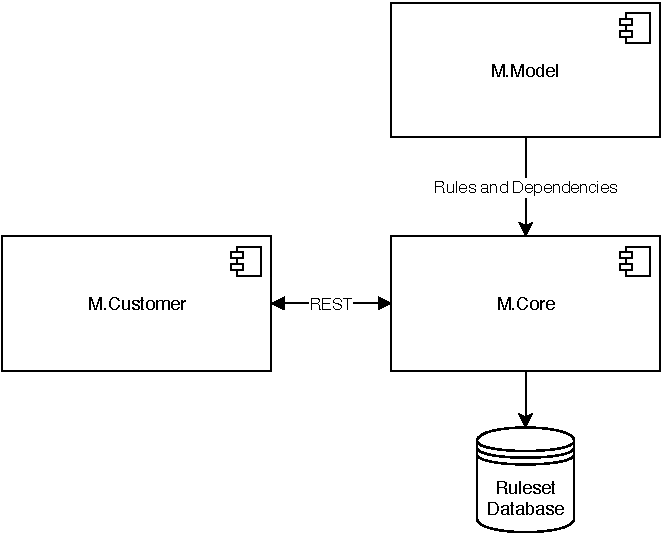
\includegraphics{./figures/50_design_and_implementation/MerlinConfigurator.pdf}
    \caption{Architecture of Configurator Merlin \cite[Fig. 4.1]{raabKollaborativeProduktkonfigurationEchtzeit2019}}
    \label{fig:DesignImplementation:ConfiguratorMerlin}
\end{figure}

\section{CAS Group-Configurator}
\label{sec:DesignImplementation:GroupConfigurator}

\citeauthor{raabKollaborativeProduktkonfigurationEchtzeit2019}'s \cite{raabKollaborativeProduktkonfigurationEchtzeit2019} extends CAS Merlin Configurator in his thesis to allow simultaneous configuration. The extended architecture is shown in \autoref{fig:DesignImplementation:CollaborativeConfiguratorMerlin}.
He only makes changes to M.Customer which is renamed to M.Collab-Customer and introduces a new component M.Collab.

\begin{description}
    \item[M.Collab] is a node.js server application that communicates with M.Core via REST-API and with M.Collab-Customer via WebSocket. It sits in between M.Collab-Customer and M.Core and handles all processing regarding collaborative configuration.
    \item[M.Collab-Customer] a modified version of M.Customer that does all communication via WebSocket and does communicate with M.Collab instead of M.Core.
\end{description}

\begin{figure}
    \centering
    \includegraphics{./figures/50_design_and_implementation/MerlinCollaborativeConfigurator.pdf}
    \caption{Architecture of Collaborative Configurator Merlin \cite[Fig. 4.3]{raabKollaborativeProduktkonfigurationEchtzeit2019}}
    \label{fig:DesignImplementation:CollaborativeConfiguratorMerlin}
\end{figure}


\section{Extended Configurator}
\label{sec:DesignImplementation:ExtendedConfigurator}

Extending \citeauthor{raabKollaborativeProduktkonfigurationEchtzeit2019} \cite{raabKollaborativeProduktkonfigurationEchtzeit2019} work a module called M.Recommender is added. Its aim is to provide a recommendation server that holds all the data needed for recommendations. M.Collab and M.Collab-Customer have to be modified to allow taking in preferences and to show  recommendations. The recommender engine is set up to be in a separate system which allows the easier replacement and the usage of different technologies. The extended architecture is shown in \autoref{fig:DesignImplementation:RecommenderForCollaborativeConfiguratorMerlin}.

\begin{description}
    \item[M.Recommender] is a new system that will get queried from M.Collab for recommendations, when the configuration changes. M.Recommender will return recommendations which then can be presented to users by M.Collab-Customer.
\end{description}

\begin{figure}
    \centering
    \includegraphics{./figures/50_design_and_implementation/MerlinCollabRecommender.pdf}
    \caption{Architecture of Collaborative Configurator Merlin with an added recommender system.}
    \label{fig:DesignImplementation:RecommenderForCollaborativeConfiguratorMerlin}
\end{figure}


\missingfigure{Figure showing screenshot of configurator UI}
\chapter{Evaluation}
\label{ch:Evaluation}

For one example e.g. forest example generate all possible valid configurations.

Generate groups with preferences (explicit preferences) and configuration state (which would be for example the currently existing forest).

\section{Group Types During Evaluation}
\label{sec:Evaluation:GroupTypes}

\begin{itemize}
    \item Groups shall be generated with random preferences
    \item With grouped preferences: people adhere more or less to one profile (Forest Owner, Athlete, Consumer, Environmentalist)
    \item Group of only one profile type: rather homogenous group
\end{itemize}

\section{Questions to Answer During the Evaluation}
\label{sec:Evaluation:Questions}

%\begin{itemize}
    %\item How close are recommendations of the recommender system to the ideal recommendation depending on the number of stored recommendations? The ideal configuration is the configuration that has the highest score with the given group scoring function $score_{group}$.
    %\item Is this approach practical?
%\end{itemize}

\begin{itemize}
    \item Main Question: How does the group decision differ from the individual decision (Randomly draw person from group -> satisfaction vs group score)
    \item satisfiability -> count individual score for example: above threshold 55\% as satisfied below 45\% as unsatisfied -> how many people on average satisfied
    \item How much negative impact does the configuration state have on outcome?
    \item Is one user type always worse off than another?
    \item Recommendation quality in relation to how many stored configurations.
    \item How much better is the best configuration than the average -> MMSE, RMSE, MAE ... % see: https://medium.com/@george.drakos62/how-to-select-the-right-evaluation-metric-for-machine-learning-models-part-1-regrression-metrics-3606e25beae0 or https://en.wikipedia.org/wiki/Error_metric
\end{itemize}

\section{Generating Data}
\label{sec:Evaluation:GeneratingGroups}

For the forest use case, the idea is that there are multiple types of user profiles. Each group profile is represented by a neutral, negative or positive attitude to an attribute value. Now during data generation the attitude is converted to a preference using a normal distribution. \autoref{fig:Evaluation:DataGeneration} shows how we convert the user profile to preferences.

\pgfplotsset{height=5cm,width=\textwidth,compat=1.8}
\pgfmathdeclarefunction{gauss}{2}{%
  \pgfmathparse{1/(#2*sqrt(2*pi))*exp(-((x-#1)^2)/(2*#2^2))}%
}
\begin{figure}
    \begin{tikzpicture}
        \begin{axis}[
            every axis plot post/.append style={
                mark=none, domain=0:1, samples=50, smooth
            },
            axis x line*=bottom,
            xmin=0,
            xmax=1,
            ymin=0.1,
            xticklabel style={
                /pgf/number format/precision=3,
            },
            xtick={0,0.25, 0.5, 0.75,1},
            hide y axis]
          \addplot [draw=red][very thick] {gauss(0.25,0.1)} node[text=red][above,pos=0.5] {negative};
          \addplot [draw=blue][very thick] {gauss(0.5,0.05)} node[text=blue][above,pos=0.48] {neutral};
          \addplot [draw=green!60!black][very thick] {gauss(0.75,0.1)} node[text=green!60!black][above,pos=0.5] {positive};
        \end{axis}
        \end{tikzpicture}
 \caption{Distribution of preferences for a user type.}
\label{fig:Evaluation:DataGeneration}
\end{figure}

These user profiles can be used to generate rather homogenous groups but also to create groups that have interests that are more conflicting. For completely random groups a uniform distribution is used to create more chaotic groups. The whole process is shown in \autoref{fig:Evaluation:GeneratingDataProcess}.



\begin{figure}
    \centering
    \includegraphics[width=1\textwidth]{./figures/bpmn_evaluation_input_data_generation.pdf}
    \caption{The process used for generating data for the evaluation.}
    \label{fig:Evaluation:GeneratingDataProcess}
\end{figure}
\chapter{Conclusion}
\label{ch:Conclusion}

\todo[inline]{write chapter}

Restating the aims of the study:
\begin{itemize}
    \item Proposed an approach to using item-based recommendation for group configuration
    \item Show the viability of a recommender for group-based configuration
    \item Produce prototype
\end{itemize}

\section{Summary}
\label{sec:Conclusion:Summary}

\begin{itemize}
    \item Summarising main research findings
        \begin{itemize}
            \item A group recommender for configuration is possible
            \item Show a design for a group based recommender for configuration that recommends complete configurations
            \item Works well for overall for groups
            \item proposed an offline evaluation metric
            \item Homogeneous groups have issues with a recommender that has only limited knowledge of the solution space -> 
            \item Works with subset of configuration space configuration
        \end{itemize}
    \item Suggesting implications for the field of knowledge
        \begin{itemize}
            \item Content based group  recommender approaches can be easily modified to work for group settings
            \item The prototype can be used and extended for future usage of recommenders in  
        \end{itemize}
    \item Explaining the significance of the findings or contribution of the study
\end{itemize}

\section{Limitations}
\label{sec:Conclusion:Limitations}
\begin{itemize}
    \item Recognising the Limitations
        \begin{itemize}
            \item Only looked at one use case
            \item Only offline evaluation
            \item Groups automatically generated - No real groups
            \item Group size fixed to four people
            \item Performance for bigger products not validated
        \end{itemize}
    \item Making recommendations for further research work 
\end{itemize}

\section{Further Research}
\label{sec:Conclusion:PossibleExtensions}

\begin{itemize}
    \item How to optimise such that no need to search through all stored finished configurations is necessary? Something like tree like structure to cluster elements
    \item How to model hierarchy and knowledge about product components in preferences?
    \item Letting users set preferences for product functions (e.g. for a forest a recreation function, a productive function, a protective function, etc.). How does it compare to explicitly choosing preferences?
    \item Does the assumption that the closer the configuration state is to a finished configuration, the less the satisfaction increase and the less difference among recommended configurations hold true?
    \item Validating if satisfaction correlates with theoretical metric used in this thesis
    \item Identification of too homogenous groups to use single person recommender.
    \item Test more complex products with more attributes and characteristics. Do they see the same effect in regards to stored configuration and recommendation quality.
    \item Evaluate different types of generating user score for configuration
    \item Larger Groups
    \item Modelling hierarchy and knowledge in group decisions for configuration
    \item Approaches towards configuration that reduce complexity and guide users for setting preferences
    \item Implicitly getting preferences
\end{itemize}




%% --------------------
%% |   Bibliography   |
%% --------------------

%% Add entry to the table of contents for the bibliography
\printbibliography[heading=bibintoc]

%% ----------------
%% |   Appendix   |
%% ----------------
\appendix
\iflanguage{english}
{\chapter{Appendix}}    % english style
{\chapter{Anhang}}      % german style
\label{chap:appendix}


%% -------------------
%% | Example content |
%% -------------------
\section{First Appendix Section}
\label{sec:appendix:FirstSection}
		
\setcounter{figure}{0}


\dots
%% ---------------------
%% | / Example content |
%% ---------------------



\end{document}
